%\documentclass{article}}
%
%\begin{document}
\documentclass[class=article, crop=false]{standalone}
\usepackage{00_Preamble/frr_preamble}
\usepackage{graphicx}
\usepackage[table,xcdraw]{xcolor}
\usepackage[normalem]{ulem}
\usepackage{longtable}
\usepackage{hyperref}
\usepackage{float}
\usepackage{graphics}
\usepackage{adjustbox}
\usepackage{placeins}

\begin{document}
	\section{Safety}
%	Safety and Environment (Vehicle and Payload)
%	Update the Personnel Hazard Anlysis, the Failure Modes and Effects Analysis, and the Environmental Hazard Analysis to include:
%	Finalized hazard descriptions, causes, and effects for the rocket the team has built
%	Note: These sections can change from CDR to FRR if there are design related changes made as a result of Sub-scale and Full-scale test flights, and refined modeling and analysis
%	These should identify specifically the mechanisms for the hazards, and uniquely identify them from other hazards. Ambiguity is not useful in Safety work
%	A completed list of mitigations, addressing the hazards and/or their causes
%	A completed list of verifications for the identified mitigations. This should include methods od verifying the mitigations and controls are (or will be) in place, and how they will serve to ensure the mitigation
%	Note: Be sure to discuss any concerns (especially operational, and environmental) that remain as the project moves into the operational phase of the life cycle.

		\subsection{Overview}
		\label{subsec:safety_overview}

		The VADL team takes individual, group, and project safety very seriously. As such, a safety hierarchy (depicted in Figure \ref{fig:safety_protocol_flowsheet}) has been developed to ensure that all team operations in the lab and on the launch field are verified and monitored by informed and qualified personnel, and that operations are stopped should a risk become uncontrollable.		
		\FloatBarrier
		\begin{figure}[h]
			\centering
			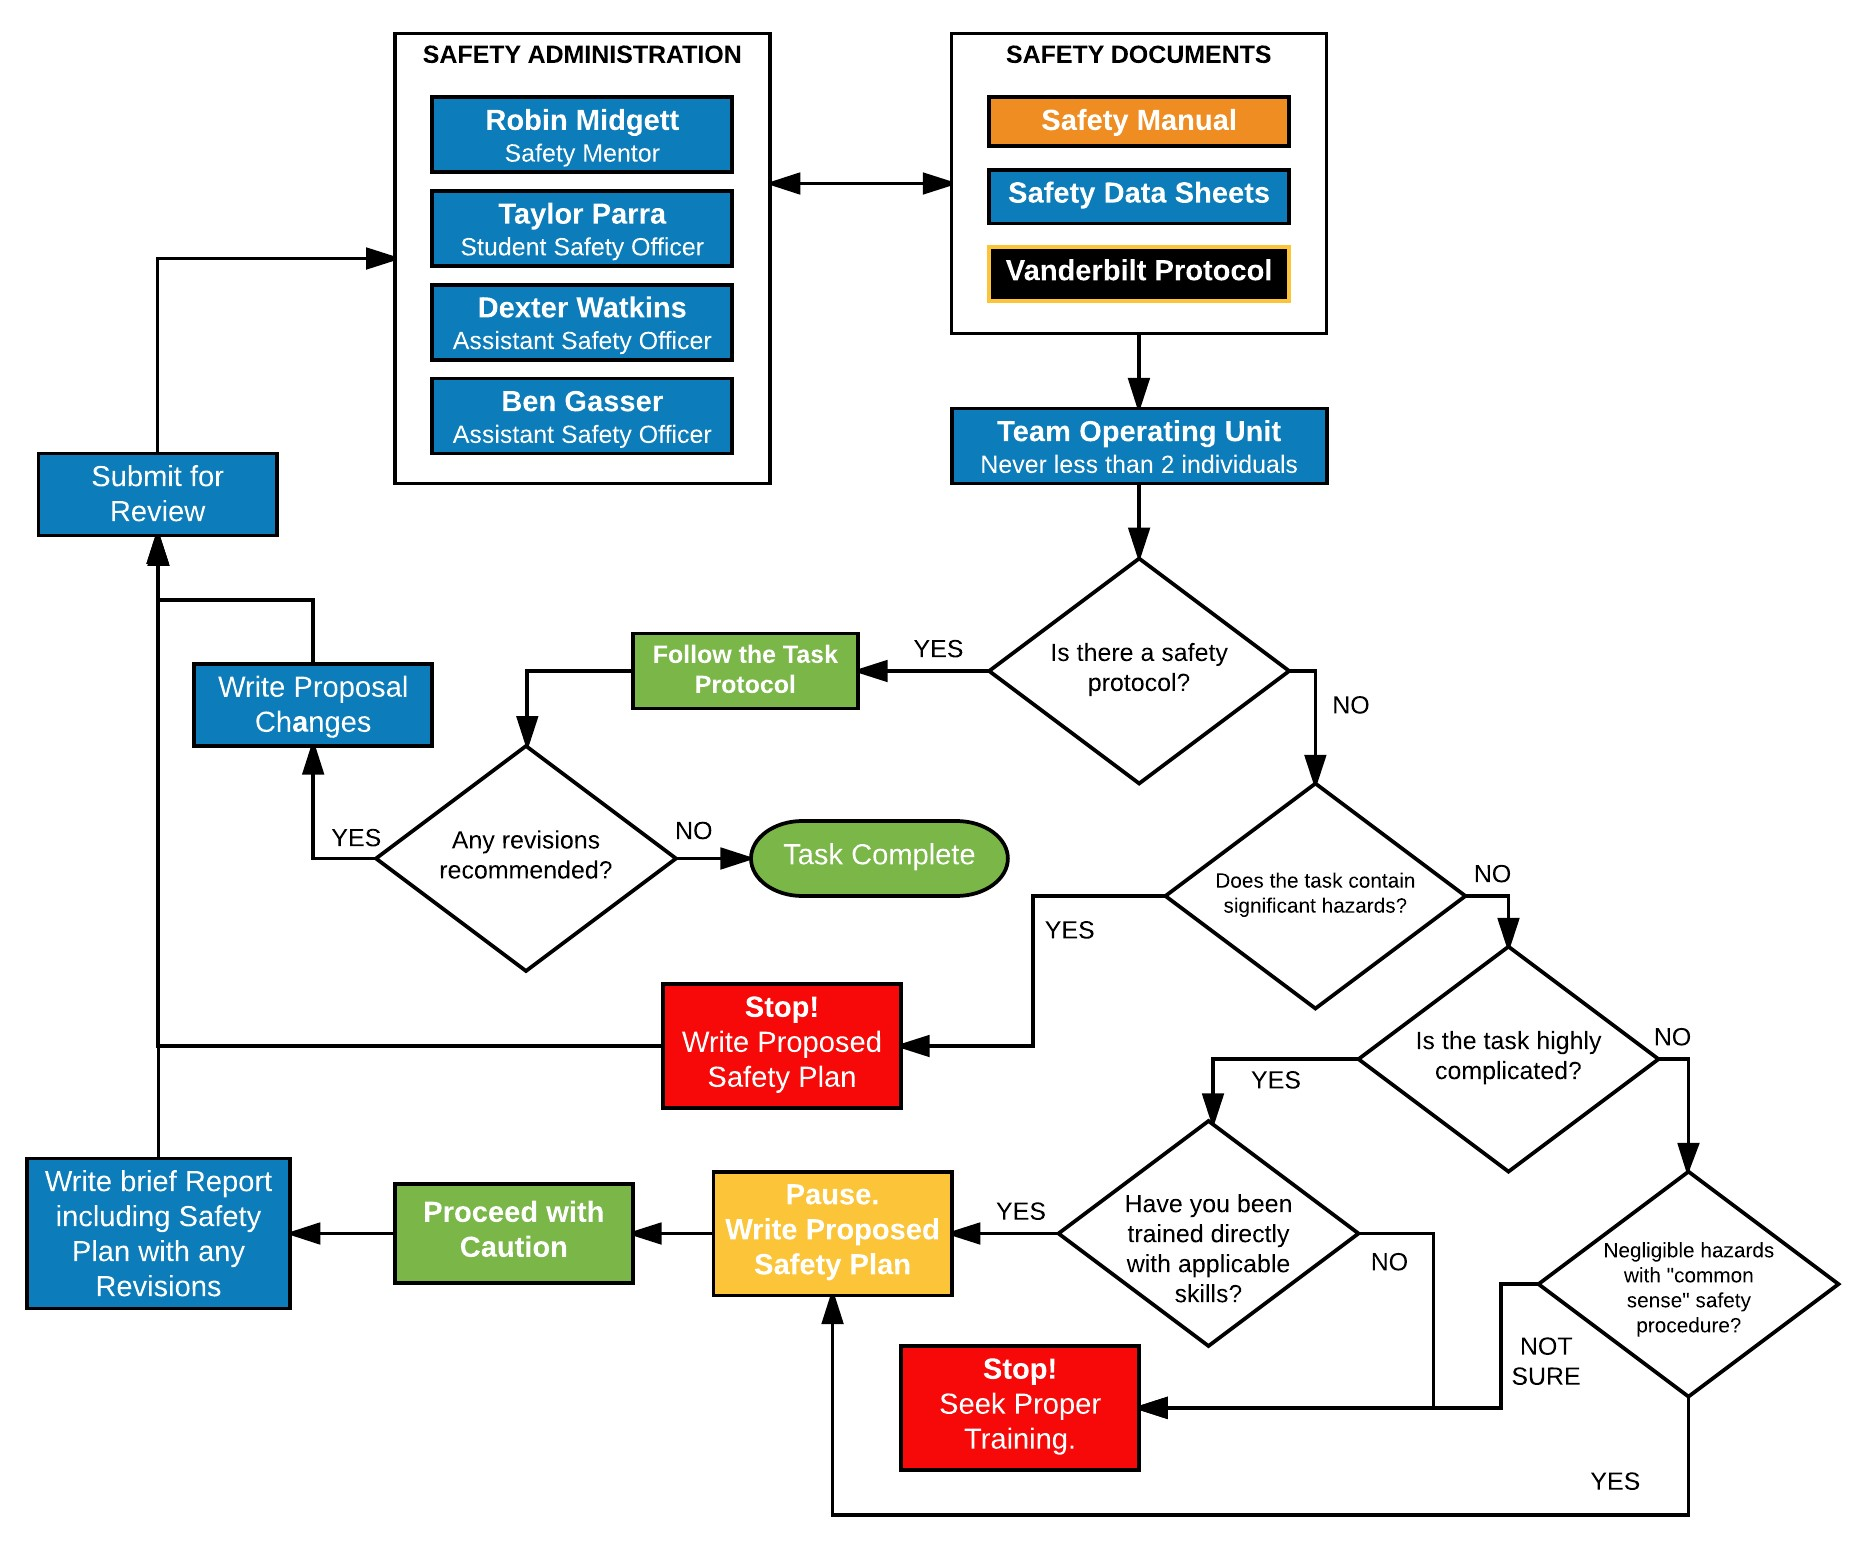
\includegraphics[width=.95\linewidth]{09_Figures/safety_protocol_flowsheet.jpg}
			\caption{Vanderbilt Aerospace Design Laboratory Safety Protocol}
			\label{fig:safety_protocol_flowsheet}
		\end{figure}
		\FloatBarrier
		
		The top level contains a four-person Safety Administration and the Safety Documents. Robin Midgett (Safety Officer; NAR II), Taylor Parra (Student Safety Officer), Dexter Watkins (Assistant Safety Officer; NAR I) and Ben Gasser (Assistant Safety Officer; NAR II) are responsible for management of the safety materials and maintain the authority to make substantive changes to the protocols and safety documentation as needed. They are also vested with the power to make go and no-go decisions for the team when new processes or procedures are required.
		\bigbreak
	
		In accordance with the Safety Hierarchy, all procedures will be performed by a Team Operating Unit (TOU). For the purposes of safety and accountability, a TOU will never consist of fewer than two individuals. All TOUs are informed by the Safety Administration and Safety Documents and are expected to pause prior to beginning any task to ask the questions outlined in Figure \ref{fig:safety_protocol_flowsheet}. 
		\bigbreak
		
		This team structure offers a significant safety net while also encouraging safety to each individual. Operating under this safety hierarchy and in TOUs ensures that every team member plays a role in hazard recognition and accident avoidance, and ensures that hazards and risks are identified and addressed early, often, and repeatedly. In addition, the common objective of safety encourages team unity, creative thinking, and problem solving skills that will promote individual and team success throughout the Student Launch competition and in students' future careers. 
	
\bigbreak

		\subsection{Safety and Environment: Hazard Analysis}
		\label{subsec:hazard_analysis}
		\subsubsection{Risk Assessment Matrix}
		\label{subsec:risk_assessment_matrix}
	
	A risk assessment matrix (see Figure \ref{fig:risk_assessment_matrix}) is used to categorize and rank risks according to the likelihood of occurrence and severity of consequence, so that particularly dangerous risks may be identified. An event's likelihood of occurrence is assigned a rating of 1, 2, 3, 4, or 5, corresponding to the designation of rare, unlikely, moderate, probable, and very likely, respectively. Similarly, an event's severity of consequence is given a rating of A, B, C, D, or E, corresponding to the designation of trivial, minor, moderate, high, or critical, respectively. When these two scales are crossed in a matrix, the resulting combinations provide enlightening information in terms of the risk level. Low alphanumeric combinations represent typically negligible risk, while high alphanumeric combinations indicate much larger risks. Color-coding has also been included in the matrix to visually depict extent of risk. Events that fall within squares highlighted in green are considered low risk and require no mitigation or have no reasonable means of mitigation. In other words, "green" risks either occur infrequently or assume low consequence, such that serious consideration to mitigate the risk is not necessary. Similarly, squares highlighted in yellow contain events with moderate risk that should be mitigated, but the overall risk posed to the mission and general safety has been deemed acceptable. "Yellow" risks are more serious than "green" risks and could result in nontrivial consequences for the success of the mission or to the safety of those involved. However, this category of risk does not necessarily represent no-go situations once potential mitigation strategies have been evaluated and implemented. The third and most critical category is highlighted in red, signifying events that pose hazardous and unacceptable risks to either mission success or personal safety. Without exception, "red" risks must be mitigated to a "yellow" or "green" level before the rocket and payload are considered safe for launch.
	
		\FloatBarrier
		\begin{figure}[h]
			\centering
			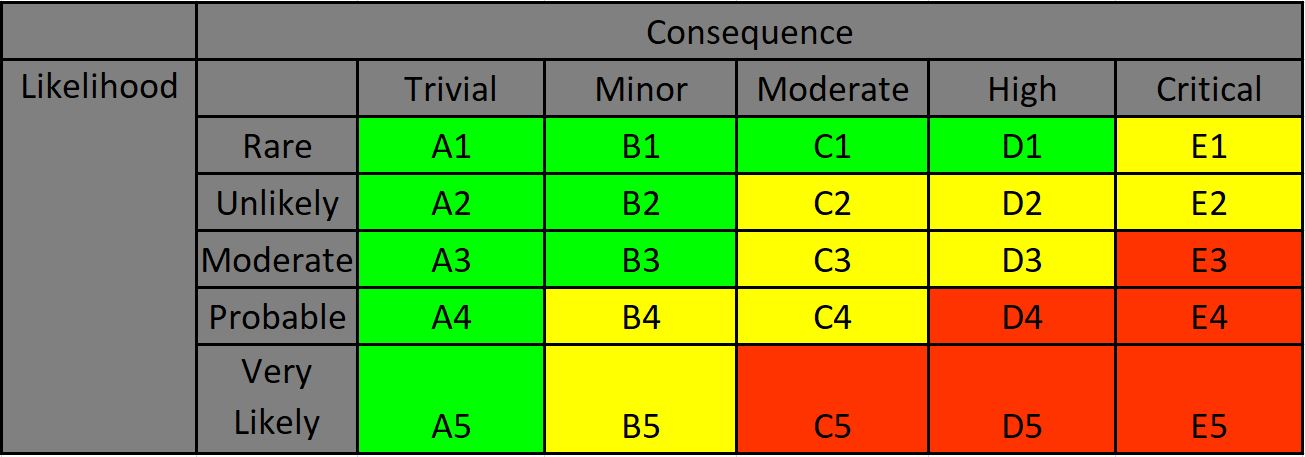
\includegraphics[width=0.9\linewidth]{09_Figures/risk_assessment_matrix.jpg}
			\caption{Risk Assessment Matrix}
			\label{fig:risk_assessment_matrix}
		\end{figure}
		\FloatBarrier
		
		\pagebreak
		
		The explicit meanings of each of the rating designations are outlined as follows:
	
		\bigbreak
	
		\textbf{Likelihood of Occurrence}
		\begin{itemize}
			\item 1 (Rare) - Probability of occurrence is almost non-existent. Mitigation need only exist for the most critical risks.
			\item 2 (Unlikely) - Probability of occurrence is very low, but does exist. Mitigation should exist for high-risk consequences.
			\item 3 (Moderate) - Probability of occurrence is moderate. Mitigation efforts should exist for all risks resulting in greater than minor consequence.
			\item 4 (Probable) - Occurrence is more likely than not. Mitigation efforts should occur for all but the most trivial consequences.
			\item 5 (Very Likely) - Occurrence is to be expected. Mitigation is required for all but the most trivial consequences.
		\end{itemize}
	
		\textbf{Severity of Consequence}
		
		\begin{itemize}
			\item A (Trivial) - Occurrence of risk results in no effect on rocket/payload performance or safety of all persons involved. No mitigation is needed.
			\item B (Minor) - Occurrence of risk results in minor damage that is either easily reparable or has no effect on rocket/payload performance. No risk for injury to persons involved. Mitigation efforts should exist for the most likely risks.
			\item C (Moderate) - Occurrence of risks results in some damage to rocket/payload that could negatively affect performance and/or result in minor injury to persons involved. Mitigation efforts should exist for most risks.
			\item D (High) - Occurrence of risk results in major damage to rocket/payload that will negatively affect performance and/or result in serious injury to persons involved. Mitigation efforts should exist for all but the rarest risks.
			\item E (Critical) - Occurrence of risk results in catastrophic damage to rocket/payload that will eliminate performance capability and/or result in serious injury/death to persons involved or bystanders. Mitigation is necessary.
		\end{itemize}
		
		\textbf{Combined Rating}
	
		\begin{itemize}
			\item Green (Low) - Risk falls within an acceptable range of probability and consequence. Mitigation strategies should be implemented if possible but are not mission critical.
			\item Yellow (Moderate) - Risk may or may not be acceptable. Risk should be evaluated thoroughly for potential mitigation strategies.
			\item Red (Critical) - Risk has an unacceptable level of likelihood and consequence. Mission should not proceed until viable mitigation strategies are created and implemented.
		\end{itemize}
		
		All risks recognized by members of the team have been recorded and evaluated by the Student Safety Officer. The results are compiled in the following risk assessment tables, wherein each risk has been outlined along with possible causes, overall effect to the rocket/payload, verified mitigation strategy, and two risk assessment ratings for pre- and post-mitigation that have been colored accordingly for easy comparison. These ratings are abbreviated RR and PMRR, respectively. The evaluated risks, which span all aspects of project management, construction and launch day, have been organized into the following categories: Personnel, Propulsion Failure Modes, Payload Failure Modes, Recovery System Failure Modes, Vehicle Failure Modes, Environmental Concerns and Project Management.
		\bigbreak
	%\documentclass{article}}
%
%\begin{document}
\documentclass[class=article, crop=false]{standalone}
\usepackage{00_Preamble/frr_preamble}
\usepackage{graphicx}
\usepackage[table,xcdraw]{xcolor}
\usepackage[normalem]{ulem}
\usepackage{longtable}
\usepackage{hyperref}
\usepackage{float}
\usepackage{graphics}
\usepackage{adjustbox}
\usepackage{placeins}

\begin{document}
		\subsubsection{Personnel Hazard Analysis}
		\label{subsubsec:personnel_hazard_analysis}
			Personnel safety is of utmost importance in all construction, testing, and launch operations. Use of any equipment or chemicals requires a thorough understanding of the safety protocol and mitigation strategies for preventing and reducing the consequences of a potential failure.
			\begin{footnotesize}	
		\begin{longtable}{|L{0.12\linewidth}|L{0.12\linewidth}|L{0.11\linewidth}|C{0.05\linewidth} |L{0.22\linewidth}|L{0.16\linewidth}|C{0.10\linewidth}|}
		
			\caption{Personnel Hazard Risk Assessment}			\label{table:personnel_hazard_risk_assessment}\\ 
			\hline
			\rowcolor[rgb]{ 1,  1,  1} \textbf{Risk} & \textbf{Cause} & \textbf{Effect} & \textbf{RR} & \textbf{Mitigation Strategy} & \textbf{Verification of Mitigation} & \textbf{PMRR} \\ \hline
			\endfirsthead
			
			\caption*{Personnel Hazard Risk Assessment}\\ 
			\hline	
			\rowcolor[rgb]{ 1,  1,  1} \textbf{Risk} & \textbf{Cause} & \textbf{Effect} &  \textbf{RR} & \textbf{Mitigation Strategy} & \textbf{Verification of Mitigation} & \textbf{PMRR} \\ 
			\hline
			\endhead
			
			\rowcolor[rgb]{ 1,  1,  1} \multicolumn{7}{|c|}{\textcolor[rgb]{ 0, 0, 0}{\textbf{Shop Safety}}} \\ \hline
			Electric shock & Static build-up on equipment handler & Destruction of electrical components; black powder explosion & \cellcolor[rgb]{ 1,  0,  0} E3 & Handlers of sensitive equipment will ground themselves to discharge static build-up. Furthermore, all high voltage components will be properly marked as \textcolor{red}{``HIGH VOLTAGE"} and locked while in use. & Consultation of shop safety guidelines
			& \cellcolor[rgb]{ 1,  1,  0} E1 \\
			\hline
			Lacerations or cuts from machines and tools & Improper use of machines/ equipment & Injury potentially requiring medical attention & \cellcolor[rgb]{ 1,  0,  0} E3 & All team members performing potentially hazardous operations will be properly trained. At least two members must be present for hazardous operations. & Consultation of safety protocol flowchart
			& \cellcolor[rgb]{ 1,  1,  0} D2 \\
			\hline
			Black powder explosion/ ignition while handling & Accidental connection to voltage source; Static discharge & Hearing damage; Disorientation; Personal injury & \cellcolor[rgb]{ 1,  0,  0} E3 & Black powder handlers will only work with small amounts at a time and ground themselves prior. & Consultation of SDS
			& \cellcolor[rgb]{ 1,  1,  0} E1 \\
			\hline
			Getting caught in a machine & Loose fitting clothing or jewelry; long hair not tied back & Potential for serious injury or death & \cellcolor[rgb]{ 1,  0,  0} E3 & Those performing machining operations will never wear loose fitting clothing or jewelry. All long hair must be tied back. & Consultation of shop safety guidelines and safety protocol flowsheet & \cellcolor[rgb]{ 1,  1,  0} E1 \\
			\hline
			Eye contact with chemicals or particulates; exposure to arc from arc-weld & Improper handling of chemicals & Discomfort and/or vision impairment & \cellcolor[rgb]{ 1,  1,  0} D3 & Appropriate eye protection will be worn for all activities involving machinery, chemicals, and welding. & Consultation of SDS, PPE: eye protection & \cellcolor[rgb]{ .6,  .8,  0} D1 \\
			\hline
			Prolonged exposure to loud machinery & Prolonged operation of heavy machinery & Disorientation and/or hearing loss & \cellcolor[rgb]{ 1,  1,  0} D3 & Hearing protection will be worn when operating heavy machinery. & PPE: hearing protection & \cellcolor[rgb]{ .6,  .8,  0} D1 \\
			\hline
			Physical contact with hot surfaces & Leaving soldering iron on; touching welded parts immediately after welding & Burns & \cellcolor[rgb]{ 1,  1,  0} D3 & All heat-producing tools will be turned off when not in use. Heat-resistant gloves will be worn when handling hot parts. Chemicals will be stored and handled safely. & Consultation of shop safety guidelines
			& \cellcolor[rgb]{ 1,  1,  0} D2 \\
			\hline
			Inhalation of chemical fumes or carbon fiber particulates & Improper handling of chemicals & Discomfort and/or damage to lungs & \cellcolor[rgb]{ 1,  1,  0} D3 & Volatile chemicals will only be handled in well-ventilated rooms and under a fume-hood when possible. A respirator will be worn when cutting, drilling, and sanding carbon fiber. & Consultation of SDS before use; PPE: eye protection, respirator & \cellcolor[rgb]{ .6,  .8,  0} D1 \\
			\hline
			Contact with flying debris from machining operations & Standard or improper tool use & Burns, abrasions, irritation of eyes or skin & \cellcolor[rgb]{ 1,  1,  0} C3 & Closed-toed shoes and long pants will be worn at all times in the shop. All members present during cutting operations will wear eye protection. & PPE: clothes that cover the body, eye protection & \cellcolor[rgb]{ 1,  1,  0} C2 \\
			\hline
			Contact with falling tools/parts & Improper storage of tools/parts & Personal injury & \cellcolor[rgb]{ 1,  1,  0} C3 & All team members will wear closed-toed footwear and long pants while machining in the shop. & Consultation of shop safety guidelines involving cleanup; PPE: clothes that cover the body & \cellcolor[rgb]{ 1,  1,  0} C2 \\
			\hline
			Tripping over loose cords & Long power cords/wires being run across the shop floor & Personal injury & \cellcolor[rgb]{ 1,  1,  0} C3 & Power strips have been installed near all machines/workspaces that may require a power outlet. & Consultation of shop safety guidelines
			& \cellcolor[rgb]{ .6,  .8,  0} C1 \\
			\hline
			Exposure to chemicals/allergens & Improper handling of chemicals and known allergens & Chemical burns, irritation of skin, allergic reaction & \cellcolor[rgb]{ 1,  1,  0} C2 & Latex or vinyl gloves will be worn when handling chemicals or known allergens. & PPE: chemically resistant gloves & \cellcolor[rgb]{ .6,  .8,  0} C1 \\
			\hline
			
			\pagebreak
			\rowcolor[rgb]{ 1,  1,  1} \multicolumn{7}{|c|}{\textcolor[rgb]{ 0, 0, 0}{\textbf{Testing on the FRAME}}} \\
			\hline
			Personnel caught in motor belt & Belt plastic failure and/or improper placement in operation whilst operator is adjusting the FRAME & Potential for injury to operating personnel & \cellcolor[rgb]{ 1,  1,  0} E2 & Perform all belt operations while power is disconnected. Inspect belt before each use for damage. Stay clear of FRAME during testing operation. & FRAME was proven in by the 2016-2017 VADL Team; Following of testing procedure & \cellcolor[rgb]{ 1,  1,  0} C2 \\
			\hline
			Fall while securing nosecone interface & Unstable ladder base; unsafe practices & Potential for serious injury & \cellcolor[rgb]{ 1,  1,  0} D3 & Optimal positioning of step ladder; visual monitoring of ladder movement while in use. & Consultation of shop safety guidelines & \cellcolor[rgb]{ 1,  1,  0} E1 \\
			\hline
			Rocket dislodged & Improper axial constraint & Potential for serious injury & \cellcolor[rgb]{ 1,  1,  0} D3 & Ensure tight compression fit of top and bottom mounts; be ready to adapt setup to different vibrational situations. & FRAME was proven in by the 2016-2017 VADL Team; Following of testing procedure & \cellcolor[rgb]{ 1,  1,  0} E1 \\
			\hline
			Structural failure & Excessive vibration; joint failure & Potential for injury to operating personnel & \cellcolor[rgb]{ 1,  1,  0} D3 & Monitor construction; ensure proper joint tightness; maintain safe distance from test facility during tests. & FRAME was proven in by the 2016-2017 VADL Team; following of testing procedure to ensure structural stability of system prior to experiment deployment & \cellcolor[rgb]{ 1,  1,  0} C2 \\
			\hline
			
			\pagebreak
			\rowcolor[rgb]{ 1,  1,  1} \multicolumn{7}{|c|}{\textcolor[rgb]{ 0, 0, 0}{\textbf{Hotbox}}} \\
			\hline
			Electric shock & Improper shielding of control system & Potential for serious injury or death & \cellcolor[rgb]{ 1,  0,  0} E4 & {Follow electrical codes in wiring; maintain safe distance from hotbox while in use. Furthermore, the compartment containing high voltage electronics is marked with a warning sign and locked while the hotbox is in use.} & Consultation of safety guidelines for handling high voltage components & \cellcolor[rgb]{ .6,  .8,  0} C1 \\
			\hline
			Shop fire & Runaway heating & Potential for serious injury or death & \cellcolor[rgb]{ 1,  0,  0} E3 & PTC Thermistor used to cut off power to hotbox; webcam to monitor progress; digital thermometer included for redundancy in measurement; fire extinguishers kept in shop. & Hotbox design was proven in by the 2016-2017 VADL Team; Visual monitoring during use
			& \cellcolor[rgb]{ .6,  .8,  0} D1 \\
			\hline
			Shop fire & Improper wiring or mounting of light bulbs & Potential for serious injury or death & \cellcolor[rgb]{ 1,  1,  0} E2 & High power circuitry completed with safety officer present; fire extinguishers kept in shop. & Hotbox design was proven in by the 2016-2017 VADL Team; Visual monitoring during use
			& \cellcolor[rgb]{ .6,  .8,  0} D1 \\
			\hline
			Shop fire & Overheating of components & Potential for serious injury or death & \cellcolor[rgb]{ 1,  1,  0} E2 & Maximum temperature possible greater than temperature ratings of every part exposed to heat; fire extinguishers kept in shop. & Hotbox design was proven in by the 2016-2017 VADL Team; Visual monitoring during use; consultation of SDS for components to be heat-treated & \cellcolor[rgb]{ .6,  .8,  0} D1 \\
			\hline
			
		\end{longtable}
	\end{footnotesize}
\end{document}

	\pagebreak
	%\documentclass{article}}
%
%\begin{document}
\documentclass[class=article, crop=false]{standalone}
\usepackage{00_Preamble/frr_preamble}
\usepackage{graphicx}
\usepackage[table,xcdraw]{xcolor}
\usepackage[normalem]{ulem}
\usepackage{longtable}
\usepackage{hyperref}
\usepackage{float}
\usepackage{graphics}
\usepackage{adjustbox}
\usepackage{placeins}

\begin{document}
\subsubsection{Propulsion Failure Modes}
\begin{footnotesize}
\begin{longtable}{|L{0.12\linewidth}|L{0.12\linewidth}|L{0.11\linewidth}|C{0.05\linewidth}|L{0.22\linewidth}|L{0.16\linewidth}|C{0.08\linewidth}|}

	\caption{Propulsion Failure Modes}\label{table:propulsion_failure_modes}\\ \hline
	\rowcolor[rgb]{ 1,  1,  1} \textbf{Risk} & \textbf{Cause} & \textbf{Effect} & \textbf{RR} & \textbf{Mitigation Strategy} & \textbf{Verification of Mitigation} & \textbf{PMRR} \\
	\hline
	\endfirsthead
	\caption*{Propulsion Failure Modes}\\ \hline
	\rowcolor[rgb]{ 1,  1,  1} \textbf{Risk} & \textbf{Cause} & \textbf{Effect} & \textbf{RR} & \textbf{Mitigation Strategy} & \textbf{Verification of Mitigation} & \textbf{PMRR} \\
	\hline
	\endhead
	Propellant fails to ignite & Improper motor packing; faulty propellant grain; damage during transportation & ``Live" situation; rocket does not launch; necessary replacement & \cellcolor[rgb]{ 1,  0,  0} E3 & Proper ignition setup; safety advisor oversees motor packing by student safety officer. & Consultation of strict safety protocol regarding motor and propellant issues & \cellcolor[rgb]{ .6,  .8,  0} D1 \\
	\hline
	Premature propellant burnout & Improper motor packing; faulty propellant grain & Altitude estimate not reached; main parachute may not deploy & \cellcolor[rgb]{ 1,  0,  0} E3 & Proper motor assembly; obtain motor only from reputable source. & Static fire testing; consultation of safety protocol & \cellcolor[rgb]{ 1,  1,  0} E1 \\
	\hline
	Improper assembly of motor & Incorrect spacing between propellant grains; motor case improperly cleaned; end caps improperly secured & Motor failure; unstable flight; target altitude not reached; damage or loss of rocket & \cellcolor[rgb]{ 1,  0,  0} E3 & Ensure proper training and supervision by safety advisor for motor assembly by student safety officer. & Consultation of strict safety protocol regarding motor and propellant issues & \cellcolor[rgb]{ 1,  1,  0} E1 \\
	\hline
	Motor mount fails & Insufficient mount strength; damage during previous launch or transportation & Motor launches through rocket; damage to/loss of rocket; unstable flight & \cellcolor[rgb]{ 1,  0,  0} E3 & Proper motor mount construction; load verification testing; test launches. & Load verification testing; design analysis of motor mount; pre- and post-flight inspections of motor mount \ref{subsec:motor_installation_and_cg_operations} & \cellcolor[rgb]{ 1,  1,  0} E1 \\
	\hline
	Transportation/ handling damage & Improper protection during transportation/ handling & Unusable motor; incapable of safe launch; potential damage to/loss of rocket & \cellcolor[rgb]{ 1,  0,  0} E3 & Proper storage overseen by safety advisor and student safety officer; certified member handling. & Consultation of strict safety protocol regarding motor and propellant issues & \cellcolor[rgb]{ 1,  1,  0} E2 \\
	\hline
	Center ring failure & Unable to withstand motor force during launch; weak ring; poor seal to body and motor tube & Reduced stability; damage to/loss of vehicle & \cellcolor[rgb]{ 1,  0,  0} E3 & Proper ring size and construction; sufficiently strong materials used (6061-T6 aluminum); redundant load path design that can sustain failure of fins or centering rings and still retain motor. & Finite element modeling to verify rings to hold conservative thrust loads using von Mises failure criterion; See CDR for FEA & \cellcolor[rgb]{ 1,  1,  0} E2 \\
	\hline
	Propellant explodes & Improper motor packing; faulty propellant grain; damage during transportation & Destruction of motor casing; catastrophic failure of rocket; potential injury to personnel & \cellcolor[rgb]{ 1,  1,  0} E2 & Proper motor assembly; safety advisor oversees motor packing by student safety officer. & Consultation of strict safety protocol regarding motor and propellant issues & \cellcolor[rgb]{ 1,  1,  0} E1 \\
	\hline
	Propellant burns through casing & Improper motor packing; faulty propellant grain; damage during transportation & Loss of thrust; loss of stability; catastrophic failure of rocket & \cellcolor[rgb]{ 1,  1,  0} E2 & Proper motor assembly; safety advisor oversees motor packing by student safety officer. & Static fire testing to verify proper motor assembly
	& \cellcolor[rgb]{ 1,  1,  0} E1 \\
	\hline
	Motor tube dislodges from rocket body during launch & Failure of fin attachment, exposing motor tube connection
	& Catastrophic launch failure, uncontrolled flight & \cellcolor[rgb]{ 1,  1,  0} E2 & Thorough construction of motor tube mounting through fins. For the motor tube to tear out, the fins would have to tear through the carbon fiber body. & Design analysis of tail section structure; visual inspection of tail section pre-flight \ref{subsec:tail_section} & \cellcolor[rgb]{ 1,  1,  0} E1 \\
	\hline
	Motor is misaligned & Centering rings misaligned; fins assembled to motor tube at an angle & Unexpected flight trajectory; unstable flight & \cellcolor[rgb]{ 1,  1,  0} C4 & Careful machining of center rings on lathe with order of magnitude higher tolerance than laser cut plywood; proper assembly of tail section using centering rings and fin alignment jig. & Design analysis of motor alignment equipment; pre-flight visual inspection of motor alignment \ref{subsec:motor_installation_and_cg_operations} & \cellcolor[rgb]{ .6,  .8,  0} C1 \\
	\hline
	Motor igniter fails & Faulty or incorrect igniter & ``Live" situation; rocket does not launch; necessary replacement & \cellcolor[rgb]{ 1,  1,  0} C2 & Proper igniter selection setup; proper power source. & Adherence to safety protocol
	& \cellcolor[rgb]{ .6,  .8,  0} C1 \\
	\hline
\end{longtable}
\end{footnotesize}
\end{document}

	\pagebreak
\end{document}
